% ****** Start of file apssamp.tex ******
%
%   This file is part of the APS files in the REVTeX 4.2 distribution.
%   Version 4.2a of REVTeX, December 2014
%
%   Copyright (c) 2014 The American Physical Society.
%
%   See the REVTeX 4 README file for restrictions and more information.
%
% TeX'ing this file requires that you have AMS-LaTeX 2.0 installed
% as well as the rest of the prerequisites for REVTeX 4.2
%
% See the REVTeX 4 README file
% It also requires running BibTeX. The commands are as follows:
%
%  1)  latex apssamp.tex
%  2)  bibtex apssamp
%  3)  latex apssamp.tex
%  4)  latex apssamp.tex
%
\documentclass[%
 reprint,
%superscriptaddress,
%groupedaddress,
%unsortedaddress,
%runinaddress,
%frontmatterverbose, 
%preprint,
%preprintnumbers,
%nofootinbib,
%nobibnotes,
%bibnotes,
 amsmath,amssymb,
 aps,
%pra,
%prb,
%rmp,
%prstab,
%prstper,
%floatfix,
]{revtex4-2}

\usepackage{graphicx}% Include figure files
\usepackage{dcolumn}% Align table columns on decimal point
\usepackage{bm}% bold math
\usepackage{amssymb}
\usepackage{url}
\usepackage{amsmath}
\usepackage{siunitx}
\usepackage{txfonts} 
\usepackage{subcaption}
\usepackage{fancyhdr}
\usepackage{braket}
\usepackage{hyperref}



\begin{document}

\preprint{APS/123-QED}

\title{Toward a variational estimation of the steady state in open quantum systems using Generalized Gibbs Ensemble}


\author{Anthony Benois}



\begin{abstract}
By considering all conserved quantities, Generalized Gibbs Ensembles (GGEs) effectively characterize the steady state of an open quantum system. We use truncated GGEs as variational states to approximate the steady state of an open quantum system, and we show that in simple single-particle cases we recover the true steady state. We apply our method to a damped harmonic oscillator.
\end{abstract}



\maketitle

%\tableofcontents


% trace operator
\newcommand{\trace}[1]{\ensuremath{\mathrm{Tr}\left( #1 \right)}}
% GGEs with normalization
\newcommand{\gge}[1]{\ensuremath{\frac{{\rm e}^{#1}}{\trace{{\rm e}^{#1}}}}}
% norm
\newcommand{\norm}[1]{\ensuremath{\vert\vert\, #1 \,\vert\vert}}
\newcommand{\lindblad}[1]{\ensuremath{\mathcal{L} \, #1}}


\section{Introduction}

% \begin{enumerate}
    % \item def open Quantum system
    % \item description of open QS with Lindblad equation  (see \ref{appendix:lindblad_equation})
    % \item why steady states (+def) important in open Q. systems + ref
    % \item previous attempts: Weimer
    % \item what Weimer additionally shows (requirements) 
    % \item def von Neumann entropy (see \ref{appendix:entropy_measurement} for the relevance of this quantity)
    % \item quick note on general frame of quantum Rényi entropy
    % \item first attempt: entropy production (see \ref{appendix:min_entropy_production})
    % \item open quantum systems: Gibbs state wrong: concept of conserved quantities, thermalization, equilibration (quench)
    % \item correct framework: GGE -> def von Neumann entropy
    % \item Gogolin: ideal GGE is the time average 
    % \item pbm with conserved quantities
    % \item Wouters: GGE expressed as an optimum even with less conserved quantities
    % \item advantage of the approach: it ensures convergence of ALL POVMS
    % \item Gibbs state as thermo in closed Q Sys
    % \item generalization time-dependent GGE in open Q sys ?
% \end{enumerate}

% $\ket{\psi}$ 
% $\rho = \ket{\psi}\bra{\psi}$ 
In quantum mechanics, closed systems are described by the Schrödinger equation and states are described by a vector $\ket{\psi}$  in a Hilbert space. Their time evolution is thus unitary. On the other hand, a system is said to be open when it is not isolated from the environment. In that case, one usually rather tracks the density matrix $\rho = \ket{\psi}\bra{\psi}$, because this formalism can additionally describe efficiently statistical mixtures, intrinsic features of the open systems (because we cannot model perfectly the influence of the environment). We also consider that their time evolution is given by a quantum Markov process, which reads the Lindblad equation, also referred to as the Gorini–Kossakowski–Sudarshan–Lindblad equation :
\begin{equation}
\label{eq:lindblad_general}
\dot \rho = \mathcal{L}\, \rho \equiv - i\mkern1mu \left[ H, \rho \right] + \sum_{k=1}^{N^2-1} \gamma_k \left( L_k \rho L_k^\dag - \frac{1}{2} \{ L_k^\dag L_k, \rho \}  \right)
\end{equation}
where $\mathcal{L}$ is the Lindlblad super-operator, $L_k$ are the Lindblad operators, $H$ is the Hamiltonian, and $\gamma_k$ are the relaxation rates for the different decay modes of the open system. This equation is derived in Breuer's book \cite{breuer2002theory}.


In this mathematical framework, a quantity of interest is the state to which the system will ultimately evolve: the steady state, defined as $\dot \rho = 0$. Several methods already exist to estimate it, such as mean-field theories \cite{diehl2010dynamical, tomadin2011nonequilibrium, lee2011antiferromagnetic} or variational principles \cite{weimer2015variational}. In particular, Weimer \cite{weimer2015variational} shows that, by using the product state of single site density matrices with higher order nearest-neighbor correlations as variational state, it is possible to find a good approximation of the steady state. He also argues that any norm used in the minimization shall full fill two requirements: it must be (i) invariant under unitary transformations and (ii) unbiased.

Here we want to estimate the steady state of an open quantum system with a variational method using the Generalized Gibbs Ensembles (GGEs) as variational state. GGEs are defined as the state which maximizes the von Neumann entropy (see eqn \ref{eq:def_vN_entropy}) given a set of (quasi-) local conserved quantities \cite{gogolin2016equilibration}:
\begin{equation}
\label{eq:def_vN_entropy}
S(\rho) = - \trace{ \rho \ln \rho}
\end{equation}
\begin{equation}
\label{eq:def_GGE}
\rho_{\rm GGE} = \mathrm{argmax}_\rho \: \{ S(\rho): \\
\forall A \in \mathcal{C} : \trace{ A \, \rho} = \trace{ A \, \rho(0)} \}
\end{equation}
where $ \rho$ is the density matrix and $\mathcal{C}$ is the set of observables whose expectation value is conserved. As a result, GGEs are always \cite{gogolin2016equilibration} in the following form :
\begin{equation}
    \label{eq:shape_GGEs}
    \rho_{\rm GGE} = \gge{- \sum\limits_{A \in \mathcal{C}} \lambda_A A}
\end{equation}
where $\lambda_A$ is the Lagrange multiplier associated to the conserved quantity $A$.
In appendix \ref{appendix:entropy_measurement}, we briefly explain the relationship between the von Neumann entropy and quantum measurements to show why this quantity is of relevance. 

GGEs are good candidates for a variational principle ($\{ \lambda_A \}_{A \in \mathcal{C}}$ being the variational parameters) because of (i) the maximum entropy principle \cite{gogolin2016equilibration} and (ii) the minimization of the KL distance (see equation \ref{eq:KL_distance}) with respect to the true steady state \cite{sels2015stationary}. 
Also, \cite{lange2018time} provides numerical evidence that in some cases the time evolution is captured by time-dependent GGE. 
So, the utility of this ensemble might not only be limited to approximating the steady state of an open quantum system.

The maximum entropy principle (i) states \cite{gogolin2016equilibration} that if the expectation value of an operator $A$ equilibrates on average, then it equilibrates towards its time average, given by :
\begin{equation}
    \label{eq:max_entropy_principle}
    \overline{\trace{A \, \rho}} = \trace{A \, \omega}
\end{equation}
where $\overline{\rho}$ is the infinite time average of $\rho$, and   $\omega = \overline \rho$ is the unique quantum state that maximises the von Neumann entropy, given all conserved quantities (GGE). 
As a result, if the system equilibrates on average at all, the steady state is described by a GGE given all conserved quantities \cite{gogolin2016equilibration}. 
However, the number of linearly conserved quantities in composite systems scale exponentially \cite{gogolin2016equilibration}: as finding all of them individually is non-trivial, GGEs cannot be used as it is. 
Therefore, a GGE approximation of the steady state must consider only a limited number of conserved quantities. 

On the other hand, (ii) Dries and Wouters \cite{sels2015stationary} show that minimising the Kullback-Leibler (KL) distance (see eqn \ref{eq:KL_distance}) between the true steady state (diagonal ensemble) and the stationary density matrix of the form \ref{eq:def_GGE}, $\mathcal{C}$ being here a truncated set of conserved quantities, will naturally lead to the condition \ref{eq:wouters_conserved_quantities}:
\begin{equation}
    \label{eq:KL_distance}
    \overline{D} = \lim_{T \to \infty} \frac{1}{T} \int_0^T {\rm d}t \, D\left( \rho(t) \vert \vert \sigma \right)
\end{equation}
\begin{equation}
\label{eq:wouters_conserved_quantities}
    \trace{A \, \sigma} = \trace{A \, \rho_d}
\end{equation}
where $\sigma$ is a truncated GGE of the form \ref{eq:def_GGE}, $\rho_d$ is the diagonal ensemble \cite{sels2015stationary}, and $D\left( \cdot \vert \vert \cdot\right)$ is the KL distance.
That is, by optimising the truncated GGE state on the $\{ \lambda_A \}_{A \in \mathcal{C}}$, the latter naturally reproduces the correct expectation values for the observables included in the model.
Furthermore, Dries and Wouters \cite{sels2015stationary} also show that if a set of operators $\mathcal{C}$ is such that the associated GGE is close to the diagonal ensemble in terms of KL distance, all projection operator valued measurements (POVMs) will show small differences. 
Altogether, GGEs associated to a limited set of conserved quantities therefore reproduce correctly, with a certain accuracy, all observables when compared to the true steady state, which is exactly described by a GGE with all conserved quantities taken into account. 


%%%%%%%%%%%%%%%%%%%%%%%%%
%
% Damped harmonic oscillator
%
%%%%%%%%%%%%%%%%%%%%%%%%%

\section{Damped harmonic oscillator}

\begin{figure}[t]
    \centering
    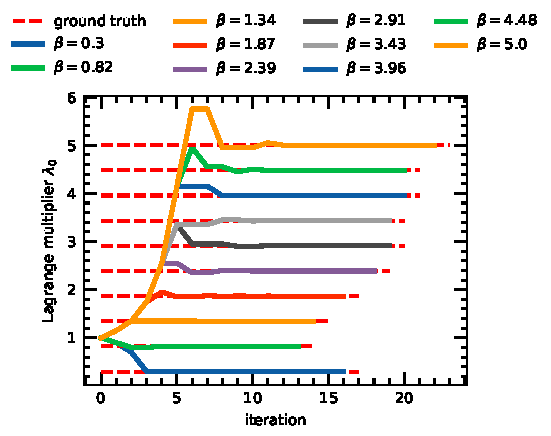
\includegraphics[scale=0.9]{figs/opti_case_1_lagr_0.pdf}
    \caption{Optimization of the GGE (ansatz 1, eqn \ref{eq:ansatz_1}): Lagrange multiplier as a function of the number of iterations. Hamiltonian: $H_0$ (harmonic oscillator, eqn \ref{eq:H_simple_harmonic_oscillator}). Lindbladian: eqn \ref{eq:toy_model}.}
    \label{fig:opti_case_1}
\end{figure}

In the present work, we lay the foundational groundwork towards establishing numerical evidence supporting the assertion that GGEs can serve as variational states for estimating the steady state of open quantum systems. 
To this end, we first focus on a single particle damped harmonic oscillator described by the Linblad equation \ref{eq:toy_model} and the Hamiltonian $H_0$ (eqn \ref{eq:H_simple_harmonic_oscillator}). 
It usually describes the damping of an electromagnetic field mode inside a cavity. We also present other Hamiltonians used later in this work, which consist on the same dynamics perturbed by a drive (eqn \ref{eq:H_drive}) or a Kerr term (eqn \ref{eq:H_kerr}).
\begin{equation}
\label{eq:toy_model}
\begin{split}
    \mathcal{L}_H \,\rho = &- i\mkern1mu \left[ H, \rho \right] \\ &+ \gamma (\bar n + 1) \left( a \rho  a^\dag - \frac{1}{2} \left\{  a^\dag   a,  \rho \right\} \right)\\ &+ \gamma \bar n  \left( a^\dag  \rho  a - \frac{1}{2} \left\{ a   a^\dag,  \rho \right\} \right)
    \end{split}
\end{equation}
where $\gamma$ is the rate of the damping of the cavity mode, $a^\dag$ and $a$ are respectively the creation and annihilation operators, and $\bar n = \left( \exp{\beta \omega_0} - 1 \right)^{-1}$ is the mean number of quanta in a mode with frequency $\omega_0$ of the thermal reservoir with inverse temperature $\beta$ (here $\omega_0=1$) .
\begin{align}
\label{eq:H_simple_harmonic_oscillator}
H_0 &=  a^\dag a \\
\label{eq:H_drive}
H_1 &=  a^\dag a + \epsilon \left( a + a^\dag \right)\\
\label{eq:H_kerr}
H_2 &=  a^\dag a + \epsilon \,  a^\dag a^\dag  a  a 
\end{align}
$\epsilon$ refers to the (small) strength of perturbation of the Hamiltonian. 
This first system is of interest because we can prove analytically (see appendix \ref{appendix:analytics_toy_model}) that it thermalises, that is, the steady state is a Gibbs state $\rho_{\rm G} \propto {\rm e}^{-\beta H}$.

\begin{figure}[t]
     \centering
     \begin{subfigure}[c]{0.45\textwidth}
         \centering
         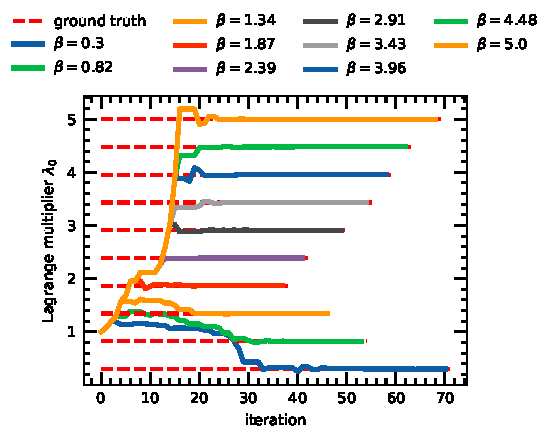
\includegraphics[scale=0.9]{figs/opti_case_2_lagr_0.pdf}
         \caption{$\lambda_0$}
         \label{fig:opti_case_2_0}
     \end{subfigure}
     \hfill
     \begin{subfigure}[c]{0.45\textwidth}
         \centering
         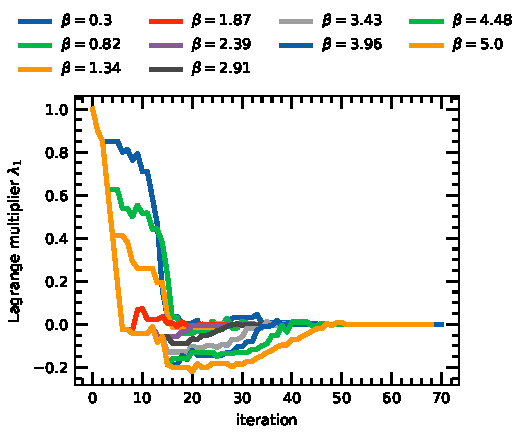
\includegraphics[scale=0.9]{figs/opti_case_2_lagr_1.pdf}
         \caption{$\lambda_1$}
         \label{fig:opti_case_2_1}
     \end{subfigure}
        \caption{Optimization of the GGE (ansatz 2, eqn \ref{eq:ansatz_2}): Lagrange multipliers as a function of the number of iterations. Hamiltonian: $H_0$ (harmonic oscillator, eqn \ref{eq:H_simple_harmonic_oscillator}). Lindbladian: eqn \ref{eq:toy_model}.}
        \label{fig:opti_case_2_all}
\end{figure}
\begin{figure}[t]
     \centering
     \begin{subfigure}[c]{0.45\textwidth}
         \centering
         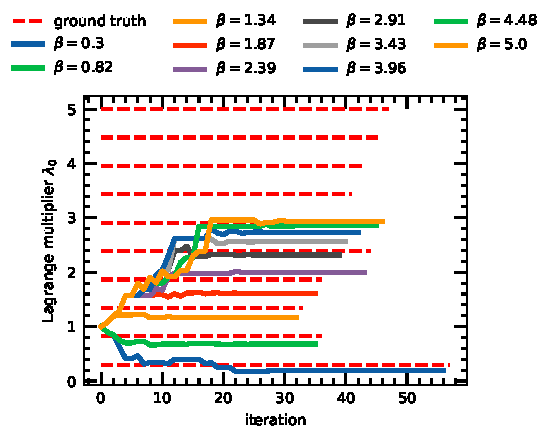
\includegraphics[scale=0.9]{figs/opti_case_3_lagr_0.pdf}
         \caption{$\lambda_0$}
         \label{fig:opti_case_3_0}
     \end{subfigure}
     \hfill
     \begin{subfigure}[c]{0.45\textwidth}
         \centering
         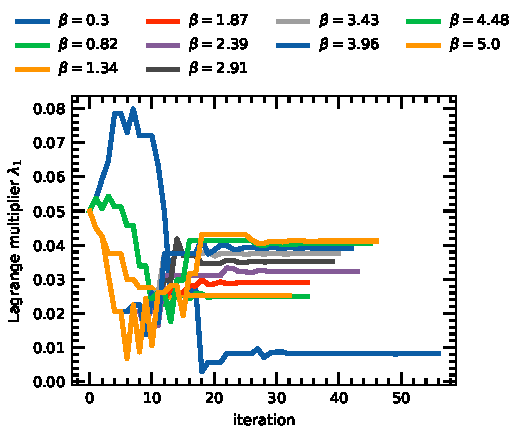
\includegraphics[scale=0.9]{figs/opti_case_3_lagr_1.pdf}
         \caption{$\lambda_1$}
         \label{fig:opti_case_3_1}
     \end{subfigure}
        \caption{Optimization of the GGE (ansatz 2, eqn \ref{eq:ansatz_2}): Lagrange multipliers as a function of the number of iterations. Hamiltonian: $H_1$ (harmonic oscillator with drive perturbation, eqn \ref{eq:H_drive}). Lindbladian: eqn \ref{eq:toy_model}. $\epsilon = 0.1$.}
        \label{fig:opti_case_3_all}
\end{figure}

To recover $\rho_G$, we successively use the following GGE ansätze:
\begin{align}
    \label{eq:ansatz_1}
    \rho_{\rm GGE \,1} &= \gge{- \lambda_0 \, a^\dag a } \\
    \label{eq:ansatz_2}
    \rho_{\rm GGE \,2} &= \gge{- \lambda_0 \, a^\dag a - \lambda_1 \,  a^\dag  a^\dag  a  a}
\end{align}
where $\{\lambda_i\}$ are the variational parametres. 
Plugged into eqn \ref{eq:toy_model}, we minimise $\norm{\dot \rho} = \norm{\mathcal{L}_{H_0} \,\rho}$ where $\norm{\cdot}$ denotes the trace norm following the recommendation of Dries and Wouters \cite{sels2015stationary}.
The optimization of ansätze $1$ and $2$ are respectively presented in figures \ref{fig:opti_case_1} and \ref{fig:opti_case_2_all}: in both cases, the procedure is able to recover the true inverse temperature (figures \ref{fig:opti_case_1} and \ref{fig:opti_case_2_0}) and to cancel extra conserved quantities (figure \ref{fig:opti_case_2_1}). Additionally, we show in figure \ref{fig:opti_case_4_all} that even by adding a small Kerr term in the Hamiltonian, the optimization of the ansatz $2$ also reproduces the correct observables.
\begin{figure}[t]
     \centering
     \begin{subfigure}[c]{0.45\textwidth}
         \centering
         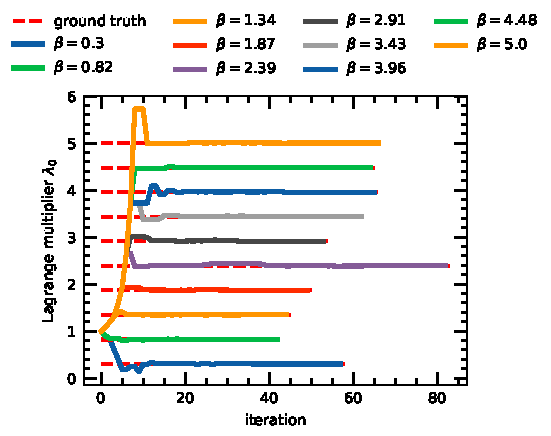
\includegraphics[scale=0.9]{figs/opti_case_4_lagr_0.pdf}
         \caption{$\lambda_0$}
         \label{fig:opti_case_4_0}
     \end{subfigure}
     \hfill
     \begin{subfigure}[c]{0.45\textwidth}
         \centering
         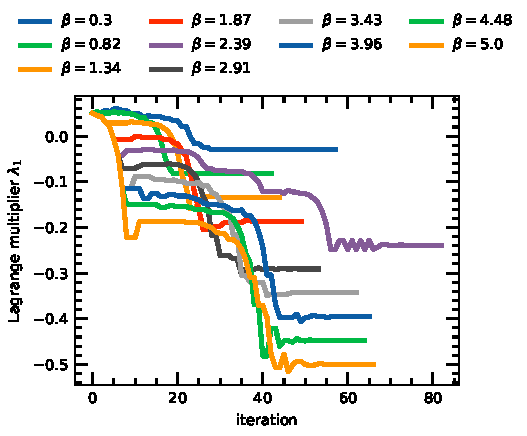
\includegraphics[scale=0.9]{figs/opti_case_4_lagr_1.pdf}
         \caption{$\lambda_1$}
         \label{fig:opti_case_4_1}
     \end{subfigure}
        \caption{Optimization of the GGE (ansatz 2, eqn \ref{eq:ansatz_2}): Lagrange multipliers as a function of the number of iterations. Hamiltonian: $H_2$ (harmonic oscillator with Kerr perturbation, eqn \ref{eq:H_kerr}). Lindbladian: eqn \ref{eq:toy_model}. $\epsilon = 0.1$.}
        \label{fig:opti_case_4_all}
\end{figure}

On the other hand, when the wrong conserved quantities are assumed in the ansatz, the model poorly reproduces the actual temperature. 
Indeed, if a small ($\epsilon = 0.1$) drive (see $H_1$, eqn \ref{eq:H_drive}) is added to the original Hamiltonian, even the ansatz $2$ is not able to recover the true temperature (see figure \ref{fig:opti_case_3_all}).


We show the performances of the ansätze regarding their respective Hamiltonian in figure \ref{fig:comp_avg_loss} by evaluating $\norm{\mathcal{L}_H \, \rho_{\rm GGE}}$ at the end of the optimization procedure: as the steady state is characterized by $\dot \rho = 0 $, this histogram directly represents the distance to the true steady state. The figure therefore simply summarizes what was inferred from the results of the previous figures showing that only the situation with a drive is not well approximated by our GGE ansatz.

\begin{figure}[h]
    \centering
    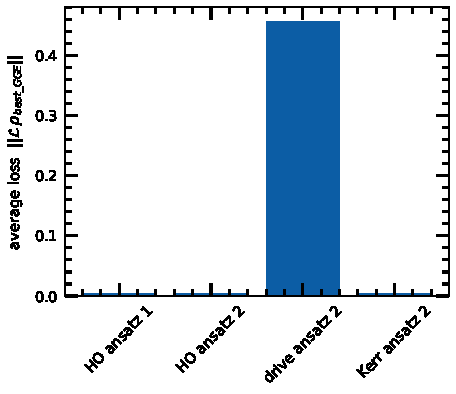
\includegraphics[scale=0.9]{figs/comp_avg_loss.pdf}
    \caption{Comparison of the losses of the optimized GGEs  in the various scenarios. The loss is the average value of $\norm{\lindblad{\rho_{\rm GGE}}}$ calculated across all true temperatures. When the Hamiltonian includes a drive, the best ansatz show significant differences from the true steady state.}
    \label{fig:comp_avg_loss}
\end{figure}




% \begin{enumerate}
    % \item link Gibbs state
    % \item goal: use GGE as variational ansatz $\to$ present all ansatze 
    % \item presentation toy model: solution is a Gibbs state (see \ref{appendix:analytics_toy_model} for the analytical derivation) $\to$ present Linbladian + all Hs
    % \item method: write as an optimization pbm, use of trace norm, optimizer
    % \item comment plots convergence
    % \item comment when temperature is too high
%     \item reproduce observables 
%     \item loss as metric 
% \end{enumerate}














% \clearpage
\section{Conclusion and outlook}

% \begin{enumerate}
%     \item Summary
%     \item Outlooks
% \end{enumerate}

In conclusion, we use GGEs as variational states to approximate the steady state of an open quantum system. 
These ensembles are formulated using predefined conserved quantities, and the parameters are their associated Lagrange multipliers.
We have applied these ideas to the damped harmonic oscillator, and in that case the variational method is able to recover the observables of the physical system.

However, the ansätze we used were strongly informed by the analytical solution. We aim to broaden the applicability of a viable variational state by expressing the conserved quantities in a more generalized form.
We also expect the method to be efficient in the multi-body case as well, which is the next step of the work.


% most likely will not want to use it.
% \nocite{*}
\bibliography{bib}% Produces the bibliography via BibTeX.

\appendix

%%%%%%%%%%%%%%%%
%
%   Lindblad
%
%%%%%%%%%%%%%%%%

% \section{Quick note on Linblad master equation}
% \label{appendix:lindblad_equation}


%%%%%%%%%%%%%%%%
%
%   Link entropy // measurements
%
%%%%%%%%%%%%%%%%

\section{Entropy and quantum measurement}
\label{appendix:entropy_measurement}

Entropy measures the lack of knowledge of a certain realisation of the state $\ket{\psi}$. Indeed, if the system is in a pure state, $S(\rho) = 0$, and $S(\rho) > 0$ otherwise. 

As a result, using Klein inequality, the von Neumann entropy can only increase for non-selective measurements (a measurement for which we do not read out the result).

However, for generalized non-selective measurements, characteristic features of open quantum systems, this is not necessarily the case. 
Indeed, let us consider a qubit described by the states $\ket{0}$ and $\ket{1}$. We build the following positive operator-valued measure (POVMs): 
\begin{align}
    \Omega_0^\dag \Omega_0 = \ket{0} \bra{0} \\ 
    \Omega_1^\dag \Omega_1 = \ket{1} \bra{1}  
\end{align}
where ($\sum_i \Omega_i^\dag \Omega_i = {\rm I}$):
\begin{align}
    \Omega_0 = \ket{0}\bra{0} \\
    \Omega_1 = \ket{0}\bra{1}
\end{align}
The associated generalized measurement of the map $\rho^M = \sum_i \Omega_i \rho \Omega_i^\dag = \ket{0}\bra{0} $ will thus always read the state $\ket{0}$, which is a pure state. In that case, $S(\rho^M) = 0$. Starting from a mixed state ($S(\rho) > 0$), the entropy decreases. Therefore, one can increase or decrease the entropy of a system with generalized non-selective measurements. 

The von Neumann entropy is thus a relevant physical quantity for the system. This is why in appendix \ref{appendix:min_entropy_production} we present our first (unsuccessful) attempt to approximate the steady state with a variational method, which is entropy production minimization.

%%%%%%%%%%%%%%%%
%
%   Entropy production
%
%%%%%%%%%%%%%%%%

\section{Minimization of entropy production}
\label{appendix:min_entropy_production}

\newcommand{\dd}[1]{\ensuremath{{\rm d}#1}}

\newcommand{\id}{\ensuremath{{\rm I}}}

We tried to characterized the steady state $\rho$ as the state which minimizes entropy production ($\delta S = 0$, $S$ being the von Neumann entropy). A variational method using this quantity would thus minimize the following quantity:
\begin{equation}
\label{eq:def_entropy_production}
\norm{\delta S} \equiv \norm{S(\rho(t+\dd{t}) - S(\rho(t))}
\end{equation}

We introduce $D(\rho, \dot \rho)$ as: 
\begin{equation}
    D(\rho, \dot \rho) = \int_0^\infty \dd{z} \, \frac{\id}{\rho + z \id} \, \dot \rho \, \frac{\id}{\rho + z \id}
\end{equation}
where $\id$ is the identity. By Taylor expanding the matrix $\ln$ \cite{adlertaylor} we get:
\begin{equation*}
    S(\rho(t + \dd{t})) - S(\rho(t)) = - \dd{t} \left( \trace{\dot \rho \ln{\rho}} + \trace{\rho \, D(\rho, \dot \rho)} \right)
\end{equation*}

Finally, the variational problem \ref{eq:def_entropy_production} reduces to finding the minimum of:
\begin{equation}
\label{eq:appendix_variational_expr_entropy_prod}
    \min \norm{\delta S} \Leftrightarrow  \min \norm{ \trace{\dot \rho \ln{\rho}} + \trace{\rho \, D(\rho, \dot \rho)} }
\end{equation}

However, expression \ref{eq:appendix_variational_expr_entropy_prod} is difficult to work with from a variational perspective, so we considered this path as a dead end.


%%%%%%%%%%%%%%%%
%
%   Entropy production
%
%%%%%%%%%%%%%%%%


% \newcommand{\dd}[1]{\ensuremath{{\rm d}#1}}

% \newcommand{\id}{\ensuremath{\text{I}}}

\section{Analytical derivation of the steady state of a damped harmonic oscillator}
\label{appendix:analytics_toy_model}

We consider the following problem:
\begin{equation}
\label{eq:toy_model_appendix}
\begin{split}
    \mathcal{L} \,\rho = &- i\mkern1mu \left[ H, \rho \right] \\ &+ \gamma (\bar n + 1) \left( a \rho  a^\dag - \frac{1}{2} \left\{  a^\dag   a,  \rho \right\} \right)\\ &+ \gamma \bar n  \left( a^\dag  \rho  a - \frac{1}{2} \left\{ a   a^\dag,  \rho \right\} \right)
    \end{split}
\end{equation}
\begin{equation}
    H =  a^\dag a
\end{equation}
where $\gamma$ is the rate of the damping of the cavity mode, $a^\dag$ and $a$ are respectively the creation and annihilation operators, and $\bar n = \left( \exp{\beta \omega_0} - 1 \right)^{-1}$ is the mean number of quanta in a mode with frequency $\omega_0$ of the thermal reservoir with inverse temperature $\beta$ (here $\omega_0=1$).

We first write the unkown steady-state density matrix $\rho$ in the basis of the oscillator eigenstates $\{\ket{n}\}$:
$\rho = \sum_{k,l} C_{kl} \ket{k} \bra{l}$. By plugging this expression into \ref{eq:toy_model_appendix}, we get the following condition on the probability amplitudes for the steady state: $C_{kl} = 0$ if $k \ne l$.

The steady-state density matrix is thus diagonal:  $\rho = \sum_{n} C_{n} \ket{n} \bra{n}$. By again plugging this expression into \ref{eq:toy_model_appendix}, we get the new condition:
\begin{equation*}
    0 = (\bar n + 1) \left( (n+1)C_{n+1} - n C_n \right) + \bar n  \left( n C_{n-1} - (n+1) C_{n-1} \right)
\end{equation*}
which admits the following solution (using $\trace{\rho}=1$): $C_n = \frac{1}{\bar n+1} \left( \frac{\bar n}{\bar n +1} \right)^n$.

As a result, $\rho = \frac{1}{1 + \bar n} \sum_n {\rm e}^{-\beta n} \ket{n} \bra{n}$, which simplifies to:
\begin{equation}
\boxed{
    \rho = \gge{- \beta H}
    }
\end{equation}









\end{document}
%
% ****** End of file apssamp.tex ******
